\documentclass[11pt]{article}
\usepackage{geometry}                
\geometry{letterpaper}                   

\usepackage{graphicx}
\usepackage{epstopdf}
\usepackage{amssymb}
\usepackage{epstopdf}
\usepackage{natbib}
\usepackage{amssymb, amsmath}
\usepackage{booktabs}
\usepackage{multicol}
\usepackage{color}           
\usepackage{hyphenat}




\DeclareGraphicsRule{.tif}{png}{.png}{`convert #1 `dirname #1`/`basename #1 .tif`.png}
\parindent 0cm

%\title{Title}
%\author{Name 1, Name 2}
%\date{date} 

\begin{document}



\thispagestyle{empty}

\begin{center}

\includegraphics[width=5cm]{ETHlogo.eps}

\bigskip


\bigskip


\bigskip


\LARGE{ 	Lecture with Computer Exercises:\\ }
\LARGE{ Modelling and Simulating Social Systems with MATLAB\\}

\bigskip

\bigskip

\small{Project Report}\\

\bigskip

\bigskip

\bigskip

\bigskip


\begin{tabular}{|c|}
\hline
\\
\textbf{\LARGE{Insert Title Here}}\\
\textbf{\LARGE{...}}\\
\\
\hline
\end{tabular}
\bigskip

\bigskip

\bigskip

\LARGE{Name 1 \& Name 2}



\bigskip

\bigskip

\bigskip

\bigskip

\bigskip

\bigskip

\bigskip

\bigskip

Zurich\\
May 2008\\

\end{center}



\newpage

%%%%%%%%%%%%%%%%%%%%%%%%%%%%%%%%%%%%%%%%%%%%%%%%%

\newpage
\section*{Agreement for free-download}
\bigskip


\bigskip


\large We hereby agree to make our source code for this project freely available for download from the web pages of the SOMS chair. Furthermore, we assure that all source code is written by ourselves and is not violating any copyright restrictions.

\begin{center}

\bigskip


\bigskip





\begin{tabular}{@{}p{3.3cm}@{}p{6cm}@{}@{}p{6cm}@{}}

\begin{minipage}{6cm}
\vspace{2mm} 
\large Tim Weber
\vspace{\baselineskip}
\end{minipage}


\begin{minipage}{6cm}
\vspace{2mm} 
\large Jan Speckien
\vspace{\baselineskip}
\end{minipage}

\begin{minipage}{6cm}
\vspace{2mm} 
\large Patrice Gobat
\vspace{\baselineskip}
\end{minipage}

\begin{minipage}{6cm}
\vspace{2mm} 
\large Lionel Gulich
\vspace{\baselineskip}
\end{minipage}


\end{tabular}


\end{center}
\newpage

%%%%%%%%%%%%%%%%%%%%%%%%%%%%%%%%%%%%%%%



% IMPORTANT
% you MUST include the ETH declaration of originality here; it is available for download on the course website or at http://www.ethz.ch/faculty/exams/plagiarism/index_EN; it can be printed as pdf and should be filled out in handwriting


%%%%%%%%%% Table of content %%%%%%%%%%%%%%%%%

\tableofcontents

\newpage

%%%%%%%%%%%%%%%%%%%%%%%%%%%%%%%%%%%%%%%



\section{Abstract}
In the recent years Texas Hold'em has been increasingly popular amongst all the age groups. Therefore our aim in this study is to research how different strategies perform against each other in a heads up. In a next step we invastigated the change in outcome if one player undergoes a learning process. \\
Hence we wrote a program using MATLAB that simulates a game of Texas Hold'em in which all feasible strategies compete against each other. In our model the strategy is represented by a single variable called risk factor that holds the wilingness of taking risks. The scale of the variable reaches from zero -extremely active- to one -extremely passive-. For the latter part one player can adjust his risk variable based on different learning algorithms, which then are compared with each other.\\
The results show that up to a risk factor around 0.4 and 0.55 the more passive player prevails. Then there is a short transition period in which both players are evenly matched. After that we can see a reversed outcome where the more active clearly dominates. Concering the learnings algorithms we observed a significant increase in the average number of games won. This indicates that with an elaborated strategy also in real Texas Hold'em an important increase in the average games won can be achieved. 

\section{Individual contributions}

The commonly used models for Texas Hold'em are mostly based on stochastical probability, which makes the implementation of algorithms highly complicated. Thus we decided to write our own simulation in order to simplify the problem using as few variables as possible. All further results and conclusions are based on our program.


\section{Introduction and Motivations}

Texas Hold’em is a variation of the card game Poker and is throughout casinos, tournaments and private people amongst the most popular of its kind. The goal of the game consists in winning all the money, or from here on called “chips” (virtual currency), from the other players at the table. As soon as someone has no more chips left, he lost and has to leave the table.
Every round consists of different stages of card dealing and then successive betting. In each stage a player can decide if and how much chips he wants to play according to some rules and by evaluating their private cards called “hand” and the cards open on the table named sequentially “flop”, “turn” and “river”.
The total amount of chips from all the players in one round is called “pot”. Every round ends with either one player getting the whole pot or sometimes with a split of the pot, if two or more players have an equivalent “score” in the end of the round. The score is the highest possible combination of the private and public cards available according to a fixed ranking.
\\
The game can be played with a varying number of people and for simplicity be subdivided into two parts: “Group stage” and “Heads up”, whereby the main difference lies in the number of people playing. In a heads up the last two remaining players are gambling for the overall victory and therefore every game of Texas Hold’em will end with a heads up.
\\
Every player has his own strategy, where some players like to play more conservative by not betting often and waiting for better cards and others play more aggressive by betting more often and trying to bluff his opponent. An important aspect of the game is the “blinds”, since they force the players to bet a fixed amount before the first cards are dealt. The blinds move forward by one player after every round. They guarantee that no player only can wait for the perfect cards and that there are always chips in the pot that can be won.
\\							
In our group we all are regular Texas Hold’em players. Therefore we all have lived through the following situation dozens of times: After every game played, a discussion is held about certain hands which should or shouldn’t be played and about the best approach on how to decide in this situations. We all agree that Texas Hold’em is about knowing your opponent and play “smarter” or “better” than him. Therefore it is not possible to have a fixed strategy. One has to be able to adjust his strategy depending on the way the opponent is playing and vice-versa.
\\
CHAME USENÄH FINDE I
After a lost game the temptation to say that it is all about the luck of certain player is great. But since there are only few professionals making a decent living of Texas Hold’em than people trying, it clearly shows that luck is not the most important factor. There are Players who can adjust their strategy way better than others.\\ 
Therefore we all often wondered what would be good strategies to best adjust to one’s opponent and in particularly how effective such strategies are. To make a valuable assumption about the effectiveness of such a strategy, one would need to play an enormous amount of games to formulate a statistically speaking valid statement. If a whole game or at least some parts of it can be simulated repeatedly under different circumstances and with varying strategies, then one could gain deeper insights into Texas Hold’em and possibly develop an applicable strategy or at least compare different approaches.

\section{Description of the Model}

\subsection{Generic Model}

\paragraph{Card replacement}
The main aspect making poker a complicated game to simulate is its use of cards. Hence our main goal was to find a model, which did not require the implementation of a deck of cards. In order to achieve a simular effect every player is given a random number, called "card value" between zero and one, representing the quality of his hand, whereas 0 would be the worst hand and 1 the best. 

\paragraph{Card value adjustment}
In poker, new cards countinuously are being unveiled, which changes the score of a hand. This aspect has to be taken in account by modifying the card value during the one hand. The impact of the new cards on the score of a hand decreases during the game. We implemented this such as in the beginning the new card value varies a lot and at the end it is more likely to stay around the old card value.

\paragraph{Risk factor}
During the game a player has to decide whether to call or to drop out of the heads up, meaning he has to evaluate if his score is good enough to continue playing. This is achieved with the so called "risk factor", which determines the character of a player. It is again a number between 0 and 1, whereas a smaller number represents a riskier player.

\paragraph{Blind}
Just as in real Poker a blind has been implemented. At the beginning of every heads up, alternately one player has to pay the blind without having seen his cards yet. In our model only a single fixed blind has been implemented, since in a heads up only the difference in  blinds is relevant.

\paragraph{Betting}
With every new card unveiled alternately the players face the decision whether to place a bet or not. Their action is determined by comparing their risk factors to their score. In total this scenario occures up to four times per hand. Each time both players can place a bet of one chip.

\paragraph{Showdown}
A showdown occurs when both players bet until the end. There the winner of a hand is evaluated and he receives all chips bet (pot). If both players have the same score the pot is split.
\subsection{Learning models}
An important part of real Texas Hold’em is to obtain an advantage by estimating the strategy of your opponent and to react accordingly.
However in this model two different approaches for learning algorithms have been chosen to optimize a players strategy:
\begin{itemize}
\item One approach was to adapt the strategy in order to minimize the losses and thus maximize the profit of a player. This model analyses a players own performance. (model Tim \& Jan)% and therefore only depends on his strategy 
\item  The other approach was to first analyse the play of the opponent and then choose the optimal strategy to best counter the other player, this of course is only possible if all outcomes for all strategies are known to the player which was the case in this model (model Patrice \& Lionel)\\
\end{itemize}
Furthermore we took the assumption, that the opponent plays strictly regular and thus no ability to learn.

\subsubsection{Threshold model}

The target of this learning model is to determine the riskfactor from player 2, which then enables to find the optimal riskfactor for player 1 for which his winning probability is increased.
Everytime a showdown is conducted player 1 gets to know the cardvalue from player 2. Because player 2 has continued the headsup with this cardvalue until the showdown it is known, that the riskfactor from player 2 has to be lower than said cardvalue. With every showdon executed the possible values for riskfactor from player 2 can be narrowed down, leaving a threshold which has to be undershot by player 2's riskfactor.


The optimal riskfactor from player 1 can then be determined with the "50 Games" Matrix. This matrix includes the winprobality for player 1 for all possible combinations of riskfactors between both players. Determining the optimal riskfactor for player 1 is then only a matter of finding the maximum in a certain area of the matrix.




\subsubsection{Bacon model}
\subsubsection{Timodel}
\subsubsection{Patrice model}

The main goal behind analysing the opponent’s way of playing is to correctly estimate his risk factor, in order to adapt one’s risk factor afterward. 
Our algorithm accomplishes this in 2 consecutive steps:
 
(Only necessary in case it is not mentioned In the introduction The opponent plays strictly regular, and every card value is equally alike.) Hence the algorithm keeps track of the number of times the opponent decides to play the first round when he is not forced to do so by the blind, called “nroundsplayed”. The ratio between this value and the total amount of rounds played called “nrounds” can then be used as a measurement to estimate the opponent’s risk factor, called “RF” as followed:
 
Formula RF= 1 –(nrounds/nroundsplayed)
 
The second part consist of finding the optimal counterpart to the risk factor estimated in above. For that reason we evaluated results obtained by simulating almost all possible combination of strategies. The data obtained indicates, that for every risk factor chosen, there is at least one optimal counterpart. After extracting these values, the algorithm can adjust the own risk factor referring to these values.
 
Advantages:
·         With an increasing number of rounds, the estimation continuously gets better
·          On a long run he will always play the most suitable strategy and optimize his return.
·         It reaches a good estimation of the opponents risk factor already after a few rounds
·         The algorythm could also use the rounds where the other player has to pay the blind by counting the number of consecutive rounds he plays and applying the same strategy just by including the models standartdeviation into the calculus. This would lead to a faster estimation of the opponents risk factor.
 
Disadvantages:
·         The algorithm requires a precise knowledge of all possible outcomes and therefore is only applicable in the same circumstances the data was obtained.
We had to take in account an estimation error as long as the number of hands played is low.








\section{Implementation}
In this chapter the Implementaion of the simulation is discribed in the following manner:
\begin{itemize}
\item Overview \& organisation of files
\item Detailed description of scripts and functions
    \begin{itemize}
    	\item adjustCardValue.m
        \item headsup.m
        \item game.m
        \item main.m
        \item ultramain.m
    \end{itemize}
\item List of all variables and their purpose
\end{itemize}

Overview and organisation of files 
%%%%%
In the poker-simulation multiple games with different strategies are played. Each game consists again of multiple parts called hands and each hand consists of up to four rounds.

\subsubsection{Organisation of files}
%%%%%
\begin{minipage}{0.48\textwidth}
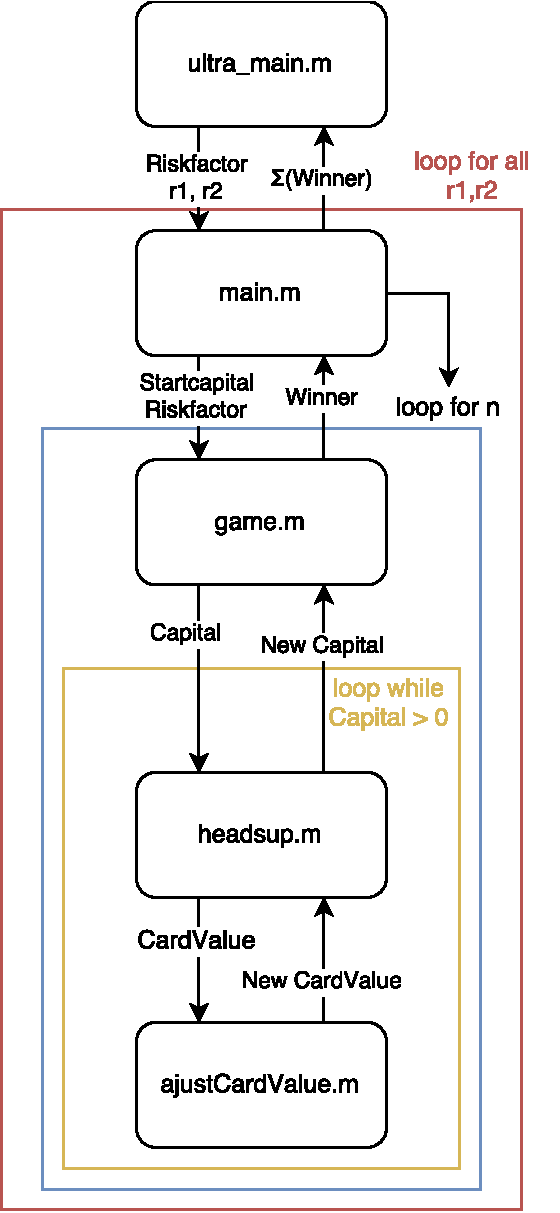
\includegraphics[width=\textwidth]{Graphics/diagram_senkrecht.pdf}
\end{minipage}
\begin{minipage}{0.48\textwidth}
For better overview the script consists of a main file that repeatedly calls a function \textit{game.m}, which simulates a complete game. The function \textit{game.m} calls a function \textit{headsup.m} that simulates one hand, until one player has run out of money (game complete). The function \textit{game.m} is called by the function{main.m}, where all relevant variabes, relevant for the simulation are defined.
After multiple tests an additional script \textit{ultramain.m} has been written to feed {main.m} with different risk-values.\\
\end{minipage}



%%%%
\begin{figure}[htbp]
	% Auff??llen des Zwischenraums
	\hfill
	% minipage mit Grafik
	\begin{minipage}{0.48\textwidth}
	% \textwidth bezieht sich nun auf die Minipage
	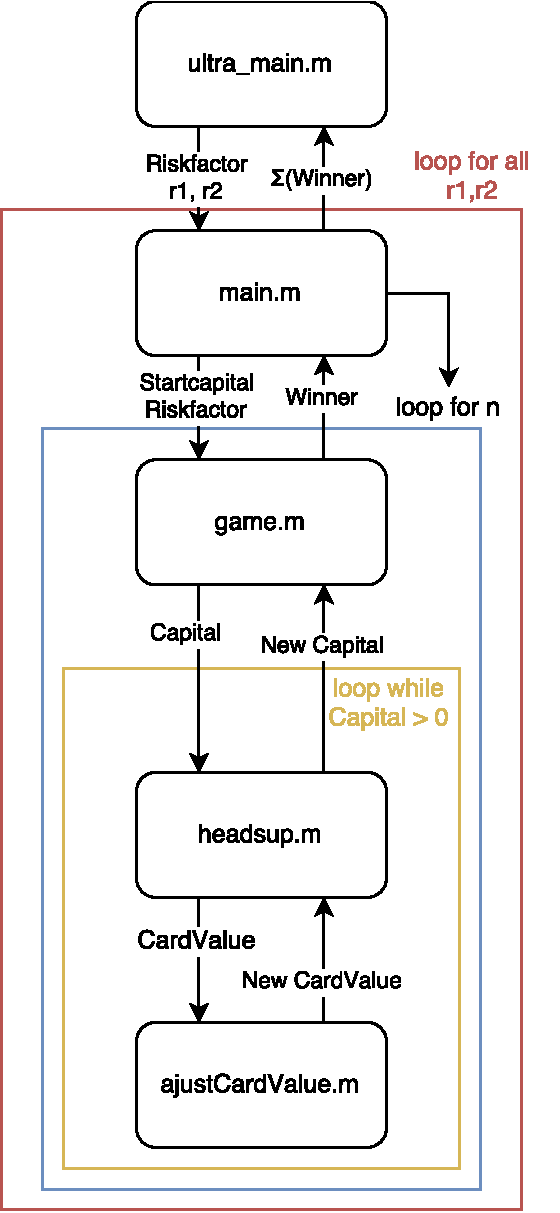
\includegraphics[width=\textwidth]{Graphics/diagram_senkrecht.pdf}
	\caption{Eine Grafik}
	\label{Bild} 
	\end{minipage}
% \caption{noch eine Caption}
	% minipage mit (Blind-)Text
	\begin{minipage}{0.48\textwidth} 
	For better overview the script consists of a main file that repeatedly calls a function \textit{game.m}, which simulates a complete game. The function \textit{game.m} calls a function \textit{headsup.m} that simulates one hand, until one player has run out of money (game complete). The function \textit{game.m} is called by the function{main.m}, where all relevant variabes, relevant for the simulation are defined.
After multiple tests an additional script \textit{ultramain.m} has been written to feed {main.m} with different risk-values.\\
	% \caption{Der Text}
	% \label{Text}
	\end{minipage}
\end{figure}

%%%
%%%%%
%For better overview the script consists of a main file that repeatedly calls a function \textit{game.m}, which simulates a complete game. The function \textit{game.m} calls a function \textit{headsup.m} that simulates one hand, until one player has run out of money (game complete). The function \textit{game.m} is called by the function{main.m}, where all relevant variabes, relevant for the simulation are defined.
%After multiple tests an additional script \textit{ultramain.m} has been written to feed {main.m} with different risk-values.\\
%
%\begin{figure}[h!]
%\centering
%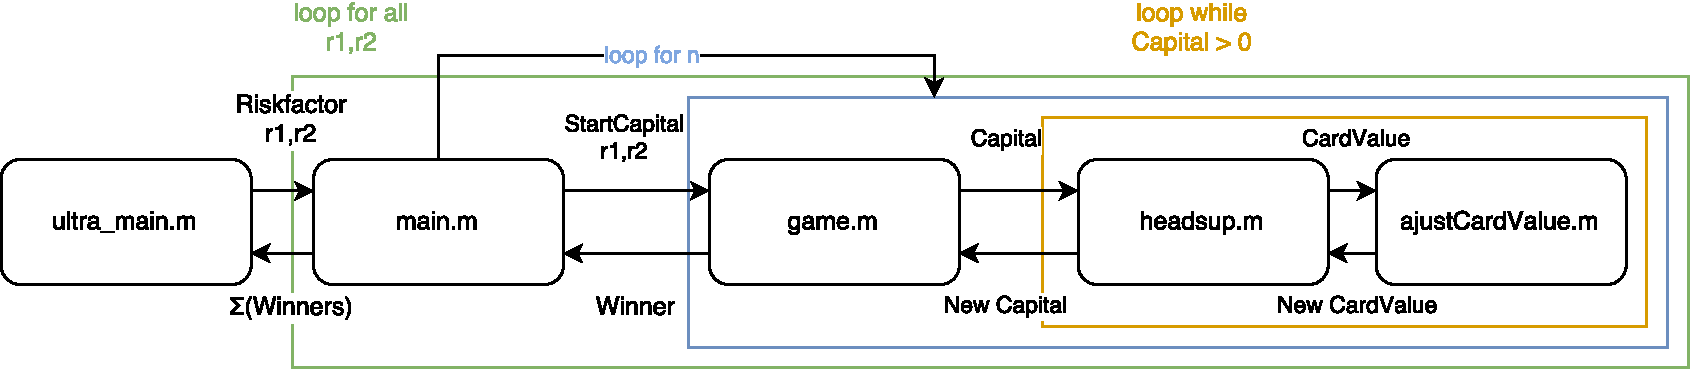
\includegraphics[scale=0.55]{Graphics/diagramm_waagrecht.pdf}
%\caption{Simplified sceme of relations of relevant scriptes\label{Abbildung}}
%\end{figure}



\subsection{adjustCardValue.m}
At the heart of this simulation lies the adjustCardValue function, which recalculates the card value of a player. Important criteria are that the cards correlate with each other, so if a player has good cards it is likely that his hand is still good when a new phase is played, but also should it be possible to for a value to reach the whole spectrum of card quality from 0 to 1. This is important because for an example in real Texas Holdem if one has a bad starting hand but with some luck to have the best hand possible after the flop. Hence every value should be possible but not with the same probability.\\
The way we implemented this mechanism is that the function receives the old card value and a number between 0 and 1 we call sigma. Then the function calculates the new value based on the normal distribution where the old card value sets the middle of the curve and the sigma determines how fast probability fades down to zero. A very high sigma means that the recalculated value has the chance to be on the whole spectrum and a very low sigma computes a new card value close to the old one.
We chose the sigma for the flop as 0.4 because there three new cards are dealt and a big variety of outcomes is needed. In the next two rounds where only one card is dealt the current card value has to be stable so the chosen sigma there is 0.2.\\
The first line of Table ??? shows the card value that needs to be recalculated and line two represents the average of a hundred new card values. This shows that with a sigma of 0.2 the average is pretty stable. The values at the top and bottom differ a little bit more because there is a set boundary at zero and one. Hence at 0.9 there are maybe as many values above this number as there are below but the ones underneath reach much lower.\\
Table two shows the highest and lowest possible resulting value of certain incoming number over a hundred played games. Whereas the first line represents the old card value, line two the highest and line three the lowest possible value. This data supports the choice of a sigma of 0.4 because every value has the potential to reach the whole spectrum.

\begin{table}[]
\centering
\caption{Old and new card values with a sigma 0.2}
\label{my-label}
\begin{tabular}{lllllllll}
0.1 & 0.2 & 0.3 & 0.4 & 0.5 & 0.6 & 0.7 & 0.8 & 0.9\\
\addlinespace
0.177 & 0.224 & 0.312 & 0.401 & 0.504 & 0.616 & 0.645 & 0.766 & 0.787 \\   
\end{tabular}
\caption{Highest and lowest possible card values with a sigma 0.4}
\label{my-label}
\begin{tabular}{lllllllll}
0.1 & 0.2 & 0.3 & 0.4 & 0.5 & 0.6 & 0.7 & 0.8 & 0.9\\
\addlinespace
0.9014& 0.9871 & 0.9972 & 0.9596 & 0.9984 & 0.9918 & 0.9992 & 0.9960 & 0.9944\\
\addlinespace
0.0045 & 0.0008 & 0.0008 & 0.0108 & 0.0035 & 0.0068 & 0.0962 & 0.0218 & 0.0071 \\   
\end{tabular}
\end{table}

\subsection{headsup.m}
The core function, on which the simulation is built around. Is called headsup.m. It simulates one poker hand and consists of up to four rounds, where players can bet money on their win. At the end of a hand a showdown determines the winner, who can increase his capital by up to four betValues, while the losers capital decreases by the same amount.\\
%sketchy \renewcommand{\arraystretch}{1.4}






\begin{center}
\begin{tabular}{c c}
Inputs & Outputs\\

\hline
CapitalP1,-P2 & CapitalP1,-P2\\

RiskfactorP1,-P2\\
BetValue\\
\end{tabular}\\
\end{center}






At the beginning of headsup each player gets a random (Card-)value Val between 0 and 1, this value replaces his two handcards in this simplified simulation. In a next step the player with a blind is forced to place this blind in the pot. The other player can decide if he wants to place an equal amount in the pot.  Of course, the placement of money in the pot reduces the capital of a player. After both players decided to play (preflop), their card-values Val are altered in the next step, that should resemble the Flop of a normal poker game. Afterwards the players get another chance to place a bet, which is followed by the river, where once more both (Card-)values are slightly altered. This is followed by a last chance to place another bet before the showdown. In which the player with the better Card-Value wins the money in the pot.

\subsection{game.m}
The function game.m is used to call the function headsup. Like in real poker game.m continues to call headsup, until one player has run out of money. To do so a while loop has been used. Game.m has the following input variables:
RiskfactorP1,-P2
CapitalP1,-P2
BetValue
The output of the function game is the winning player.
\subsection{main.m}
In the function main.m all important variables are defined and passed on the function game.
Additionally to that the variables needed to in the function main the number of games played is defined.
Ultra-main: Is an additional script used to efficiently vary risk-factor one and two and to display the results in the form of a matrix.
%%%%--------------List of Variables----------------%%%%
\subsection{List of all variables and their purpose}
\begin{itemize}

\item	\textbf{Skripte:} \textcolor{red}{Main, Game, HeadsUp} \\

\item	\textbf{playerP1, playerP2, \textcolor{red}{M}:} 
Represent the two players $|$ vector of five elements
\begin{enumerate}
	\item riskFactorP-
	\item playerP-(2) (Capital)
	\item playerP-(3) (cardValue)
	\item playerP-(4) (sum of bets placed by one player during one hand)
\end{enumerate}		
	
\item	\textbf{riskFactorP1, riskFactorP2, \textcolor{red}{M}:}  A fixed parameter between 0 and 1 that represents the willingness to play risky (strategy). A low risk-factor means the player is very venturesome and plays nearly every hand, while a high risk-factor stands for a passive player, that only plays a hand if the cards, and thus the chances of him winning, are high.\\


\item	\textbf{playerP1(2), playerP2(2), \textcolor{red}{G, H}:} Current Capital of the players. This value is set individually by \emph{startCapitalP-} at the beginning (of a game) and varies over the course of a game.\\

\item	\textbf{playerP1(3), playerP2(3), \textcolor{red}{H, A}:} Current card score of the player (combination of private and public cards). If  \emph{riskFactorP- $<$ playerP-(3)}, the player raises respectively calls\\

\item	\textbf{playerP1(4), playerP2(4), \textcolor{red}{H}:} 
Sum of a players bets during a hand, incremented by\emph{betValue}\\
	%%%%% losses
\item	\textbf{n, \textcolor{red}{M}:} Numbre of games to be played during the simulation\\

\item	\textbf{betValue, \textcolor{red}{M,H}:}Amount of chips a player can bet each round of the game\\

%%bruuchts ned, oder?
%\item	\textbf{blindOn, \textcolor{red}{M}:} Blinds ein-/ausschalten\\

\item	\textbf{blindValue, \textcolor{red}{M}:} Number of chips that has to be placed in the pot to play\\

%ebefalls unn??tig
%\item	\textbf{gameValues, \textcolor{red}{M}:} Zeilenvektor, der die Spieleinstellungen \emph{betValue, blindOn, blindValue} speichert\\

\item	\textbf{winsP1, winsP2, \textcolor{red}{M}:} Number of games won by a player, incremented by \emph{winner}\\
%sollte neu definiert werden
\item	\textbf{rounds, \textcolor{red}{Hallo HIER}:} Vektor mit Anzahl gespielte H"ande pro Spiel\\

\item	\textbf{totalRounds, \textcolor{red}{HIER}:} Gesamte Anzahl gespielte H"ande f"ur alle \emph{n} Spiele\\	

\item	\textbf{counter, \textcolor{red}{M, G HIER}:} Anzahl Runden bis ein Spieler gewinnt, hilft zum setzen von \emph{rounds} \\

\item	\textbf{winner, \textcolor{red}{M, G}:} Winner of a game, increments \emph{winsP1} \\

\item	\textbf{pot, \textcolor{red}{H}:} Amount of all bets placed during a hand. %Wird an \emph{playerP-(2)} verteilt, wenn dieser gewinnt
\\

\item	\textbf{betRounds, \textcolor{red}{HIER}:} Anzahl gespielte Runden pro Hand \\

\item	\textbf{adjustCardValueP-, \textcolor{red}{H}:}
function, that recalculates the current card-score \emph{playerP-(3)} of a player out of his private and the public cards after every action card.\\



\end{itemize}


%%%%--------------/List of Variables----------------%%%%
\subsubsection{Bacon model}
This learning algoritm analyzes the loss of the last hand, because if the last hand has been won there is no need to adapt the strategy. So after every hand one of the following scenarios take place\\
\renewcommand{\arraystretch}{1.4}
\begin{tabular}{ p{6.45cm}   p{5.1cm}  p{2.4cm}}
%\hline
Validation & Interpretation & Action\\
%\end{tabular}
\addlinespace
%\begin{tabular}{ p{6.2cm}  | p{5.1cm} | p{2.7cm}}
%\hline
CapitalP-($t+1$) $>=$ Capital($t$) &	The player had equal or better cards, or the hand has not been played&
r will not be changed \\
%\hline
\addlinespace
CapitalP-$(t+1) ==$ Calpital$(t)-4$	&	The player has lost after the showdown and is thus to agressive & \ r=r+0.012\\
%\hline
\addlinespace
Else (CapitalP- dropped by 1,2 or 3) &	The player is to passive, since it did not come to a showdown & \ R2=R2+0.003\\
%\hline


\end{tabular}

\begin{figure}[h!]
\centering
\includegraphics[scale=0.6]{Graphics/Janfigure.pdf}
\caption{The figure above shows the progression of the capital of the player using the learning algorithm starting at 1000 chips. The figure below shows the progression of the corresponding riskfactor of the same player starting at $r(0)=0.1$ against a player with a riskfactor of $r=0.7$.\label{Abbildung}}
\end{figure}

As seen in figure \ref{Abbildung} the algorithm needs around 800 hands in order to leed to a good estimation for the optimal parameter r. This leads to good results for startcapitals above 70 and to very good results at startcapitals above 300 even with a very unfavorable starting strategy like r(0)=0.1.
\\
\begin{tabular}{ p{7.2cm}  p{7.2cm}}
Advantages & Disadvantages\\
The model has a great potential for different kinds of optimization:
\begin{itemize}
\item parameters used in the model can still be optimized in order to perform quicker
\item more cases for different scenarios could be made (different action for loss of 1 and loss of two)
\item the cards that the player has could be taken into account in order to avoid a change in policy if there has just been bad luck with the cards 
\end{itemize}
 & The algorithm is based on a simplified scenario, where the only reason for a loss is besed on the strategy and never on luck. This leads in some cases to a change of policy even when this is not desired. This can be observed in the high standart deviation, even after haveing fond a well estimated r. This behavior leeds to the algorithm loosing against extreemly strong strategies due to its contious slight deviations from the optimum  riskvalue.\\ 
\end{tabular}



\section{Simulation Results and Discussion}
\begin{figure}
\begin{center}


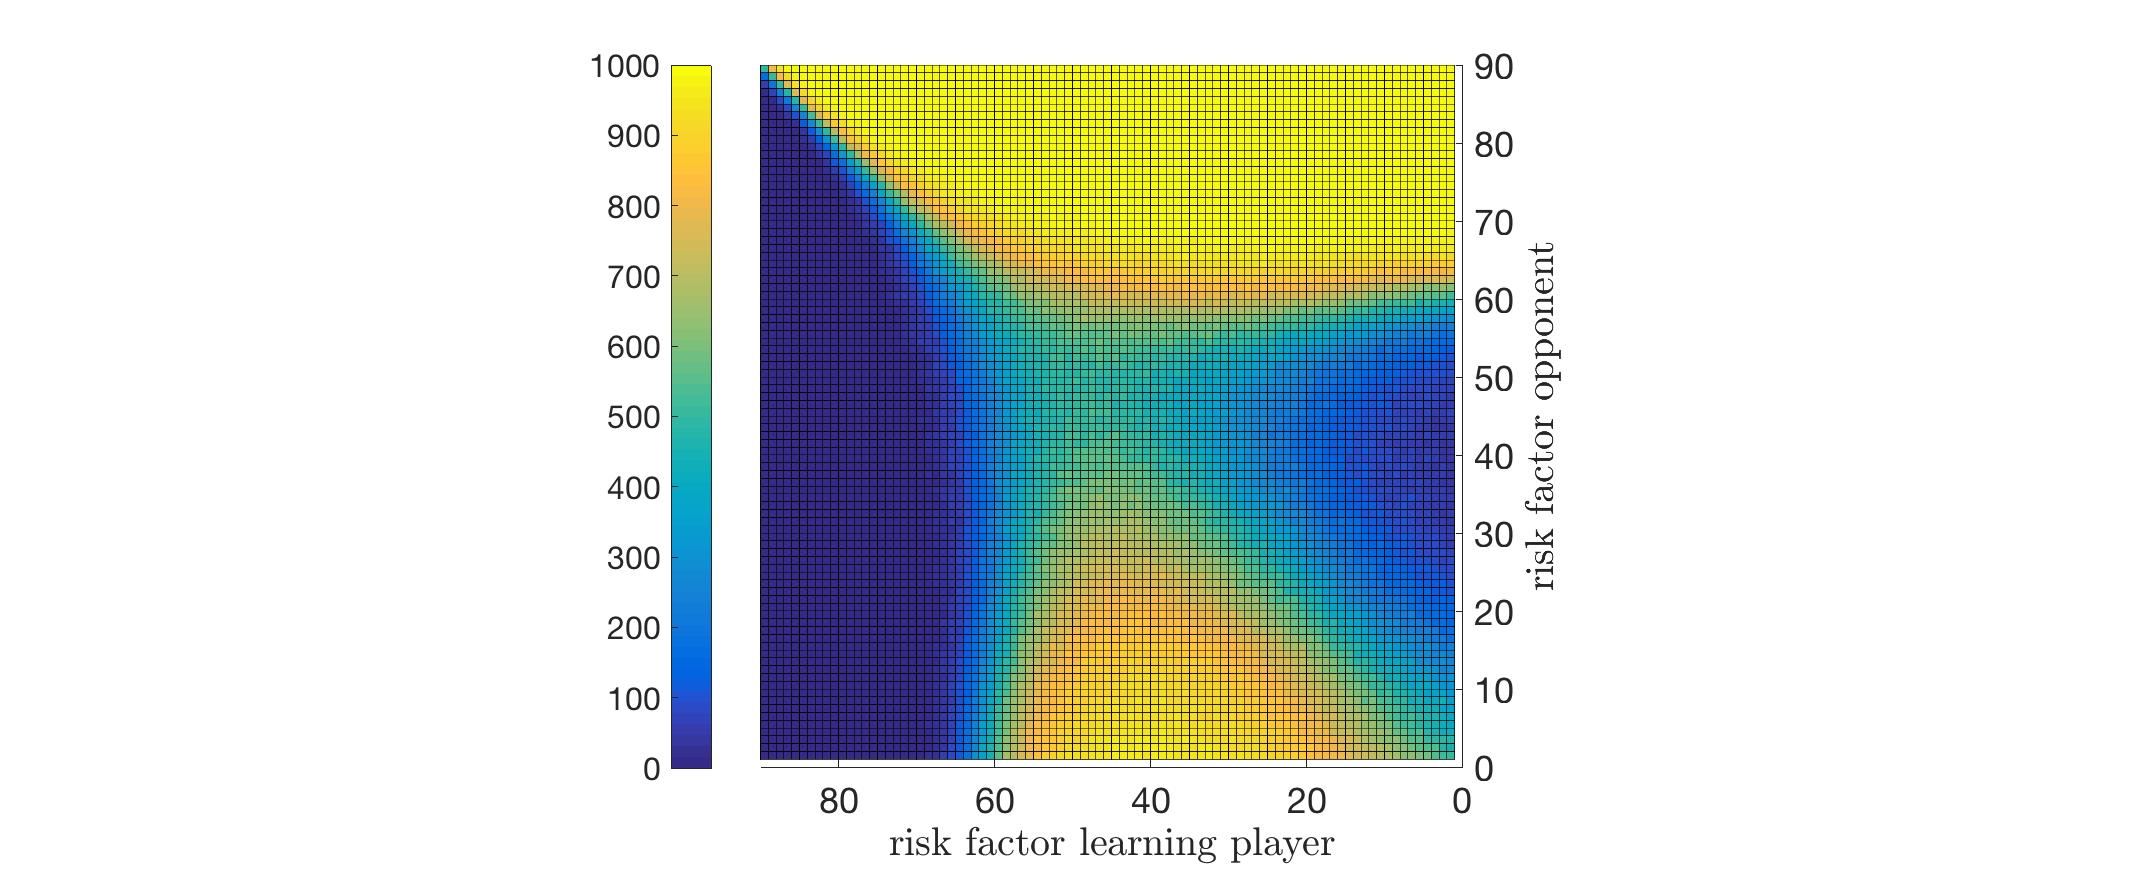
\includegraphics[scale=0.2]{Graphics/allDataPlot_BlindOn_1000Games_001Step_TopFlat.jpg}
\caption{Games won by player1 out of 1000\label{Topview of all Data}}
\end{center}
\end{figure}

\subsubsection{Results with blinds}
The figure \ref{Topview of all Data} shows how many games player1 has won out of a total of 1000, when both players started out with an equal amount of chips (50) and a fixed blind equal to the betValue of 1. The colour of every cell ($x=r1|y=r2$) shows the number of games won by Player1 with his risk factor $r1$ against player2 with a risk factor $r2$.\\
%so etzte 
On the diagonal ($r1=r2$) a green line can be seen, which shows that player1 and player2 have each won half of all games played. Around this line the games won by a player are antisymmetrically distributed, which means that both players did equally well when using the same risk factor (strategy) $r$.
A too agressive startegy ($r < 0.4$) did not perform well. When a player had a too passive strategy ($r > 0.64$) he was not able to win many games eigther, unless the opponent played very passive as well. In the case of two nearly identical strategies the slightly more passive player hs had an advantage.
If both riskfactors are between 0.45 and 0.55 the games were very balanced and not even an optimal conter-strategy did win more than 60\% of all games. An optimal risk factor against most other strategies was found to be around $r=0.5$. \\
\subsubsection{Results with blinds | Interpretation}

We translate these findings into real Texas Hold’em as follows: In General a player has to be just a little more passive than his opponent, to ensure that when he plays his hand it will be better than the one of the opponent.
Inside the Interval $[0.45 < r1,r2 < 0.55]$ where both players adopt a balanced strategy, the same applies but with less certainty of a fixed outcome. In our eyes this represents the influence of luck during Texas Hold’em. The loss of a too aggressive player is easily explained by the fact that such a player will lose a lot more often than he wins because he also playes weak hands. A too agressive player looses mianly due to the blinds because his card score often drops below his risk factor, before the showdown.


\section{Summary and Outlook}
HIER FELHT NOCH SUMMARY This project is developable in many kind of ways. We had thought of some different things we originally wanted to implement but we did not have the time to. \\
One of them was implementing a blind that would increase over time. This is how it is played in real Texas Holdem with the motive to punish passive play. Because of that it would have been interesting to observe what difference it would have made in our simulation, also since our games lasted up to over a thousand hands and this is far away from reality. \\
One could also have tweaked the capital/blind ratio in general. Possible outcomes could have been that with a certain ratio the aggressive player gets punished because his loosing hands include bigger pots, but perhaps the conservative player looses more often because games are more fast paced.\\
Another extremely interesting feature could have been giving the players the option to decide with how much money the wanted to raise the pot. Currently, one is the only option but how would the outcome of a game be if they could bet one, two or three. If that was the case, card evaluation needed to be different. A player now not only has to take his own cards in to the decision if he wants to play or drop out but also how much money his opponent has bet in this phase. Furthermore, would this change have opened the opportunity for a player to bluff his counterpart, this means pretending to have better cards then what he actually has. Now maybe the more active player gets more rewarded for his play style.\\
The possibility of checking could also have been included. Checking is doing nothing when your opponent has not bet any money. This would open different strategies, because now it is possible that a hand plays out until the end with both players checking all the way to the showdown. This variation would need a distinct playing order and that would put the one, who has to show his cards first in a showdown, into a disadvantage. All these factors could play a role in developing a winning algorithms.\\
Other variations that certainly would lead to different discoveries but would made the program much more complex are coding ''real'' cards with their actual probabilities to show up in a hand but also including more than two players which might would change the power dynamics between active and passive players.


\section{References}

\section{Appendix}
\subsection{Source Code}
\subsection{Variable documentation}
\subsubsection{Variables from generic model}




\begin{itemize}

\item	\textbf{Scripts:} \textcolor{red}{ultra\_main(um), main(m), game(g), headsUp/headsUp2(h), adjustCardValue(acv)} \\

\item	\textbf{playerP1, playerP2, \textcolor{red}{general}:} Vector with 4 entries representing all important variables from one player.
\begin{enumerate}
	\item risk factor for player
	\item capital from player
	\item card value from player, is a random number between 0 and 1
	\item total bet from player
	\item free variable for learning implementation
\end{enumerate}		
	
	
	
	
\item	\textbf{allData \textcolor{red}{um}:}  Matrix containing number of Wins from player 1 one for varying riskfactors\\
	
\item	\textbf{r1, r2 \textcolor{red}{um}:}  iteration variables representing riskfactors for players 1 and 2\\

\item	\textbf{betValue \textcolor{red}{m,h}:} represents the amount a player can bet on his win or the amount by which the pot can be increased per round per person \\

\item	\textbf{n \textcolor{red}{m}:}  iteration variable for determining how many games are being simulated, hence determining the accuracy of the monte carlo approach\\

\item	\textbf{riskFactorP1, riskFactorP2 \textcolor{red}{m}:}  variables representing the riskfactors for both players\\

\item	\textbf{startCapital \textcolor{red}{m}:} determines the capital at the beginning of the game for both players. \\

\item	\textbf{winsP1 \textcolor{red}{m}:} amount of total wins by player 1, used as output to the function main.m  \\

\item	\textbf{winner \textcolor{red}{m,g}:} stores the the winner of the game simulated: if 0 winner is player 2, if 1 winner is player 1, used as output to the function game.m\\

\item	\textbf{counter \textcolor{red}{g}:} counts amount of hands played in one game \\

\item	\textbf{decide\_who\_starts \textcolor{red}{g}:} used to determine whose turn it is to start with betting, if 0 player 2 begins, if 1 player 1 begins  \\

\item	\textbf{pot \textcolor{red}{h}:}  stores the total amount of money betted by both players\\

\item	\textbf{capP1, capP2 \textcolor{red}{}:} output variables to headsUp.m function storing the capital of the corresponding player after having played the hand\\

\item	\textbf{newRandValue \textcolor{red}{acv}:} output to adjustCardValue.m function, stores the newly generated cardvalue  \\

\item	\textbf{sigma \textcolor{red}{acv}:} theoretically the standard deviation of a normally distributed random value, here used to determine the range of adjustement for the function adjustCardValue.m \\

\end{itemize}

\subsubsection{Variables from learning models}
\paragraph{Threshold model}
\begin{itemize}
\item	\textbf{Scripts:} \textcolor{red}{ultra\_main(um), main(m), game(g), headsUp/headsUp2(h), adjustCardValue(acv), adjustRiskFactor(arf)} \\

\item	\textbf{totalCounter \textcolor{red}{m}:} used to store total amount of hands played per game  \\

\item	\textbf{playerP1(5) \textcolor{red}{g}:} stores the riskfactor of player 2 as it is currently estimated by player 1  \\

\item	\textbf{startRiskFactor \textcolor{red}{h}:} input to headsup.m function, stores the riskfactor from player 2 as estimated by player 1 before the respective hand  \\

\item	\textbf{estRiskFactor \textcolor{red}{h}:} output from headsup.m function, stores the riskfactor from player 2 as estimated by player 1 after the respective hand   \\

\item	\textbf{newRiskFactor \textcolor{red}{arf}:}  output from adjustRiskFactor.m function, stores newly generated riskfactor\\

\item	\textbf{opponentRiskFactor \textcolor{red}{arf}:} input to function adjustRiskFactor.m, currently estimated riskfactor from opponent player \\

\item	\textbf{refSurf \textcolor{red}{arf}:} two-variable function which represents amount of wins for player 1 in dependence of the respective riskfactors \\

\item	\textbf{funVector \textcolor{red}{arf}:} parameterisation of refSurf at point of opponentRiskFactor \\

\end{itemize}






\end{document}  



 
